\section[Modèle conceptuel]{Modèle conceptuel}

%\subsection{Définitions}

\begin{frame}
  \frametitle{Entité}
  \begin{itemize}
    \item Entité : population d'individus homogènes
  \end{itemize}
  \begin{center}
    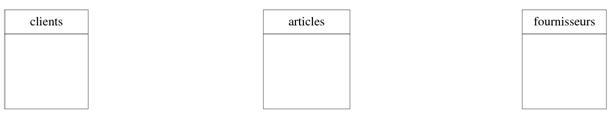
\includegraphics[width=0.9\linewidth]{entite.jpg}
  \end{center}
  \begin{itemize}
    \item Les produits ou les articles vendus par une entreprise sont de même nature (désignation, prix, etc.)
    \item[$\ra$] Ils peuvent être regroupés dans une même entité \emph{articles}
    \item Les \emph{articles} et les \emph{clients} ne sont pas de même nature (informations non homogènes)
    \item[$\ra$] On utilise deux entités distinctes
%      (un article ne possède pas d'adresse et un client ne possède pas de prix unitaire). Il
%      faut donc leur réserver deux entités distinctes : l'entité articles et l'entité clients.
  \end{itemize}
\end{frame}

\begin{frame}
  \frametitle{Association}
  \begin{itemize}
    \item Association : liaison qui a une signification précise entre plusieurs entités
  \end{itemize}
  \begin{center}
    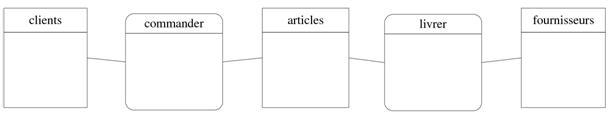
\includegraphics[width=0.9\linewidth]{association.jpg}
  \end{center}
  \begin{itemize}
    \item L'association \emph{commander} relie les entités \emph{articles} et \emph{clients}
    \item L'association \emph{livrer} relie les entités \emph{articles} et \emph{fournisseurs}
    \item L'entité \emph{clients} et relié indirectement à l'entité \emph{fournisseurs} via l'entité
      \emph{articles}
  \end{itemize}
\end{frame}

\begin{frame}
  \frametitle{Attribut}
  \begin{itemize}
    \item Attribut : propriété d'une entité ou d'une association
  \end{itemize}
  \begin{center}
    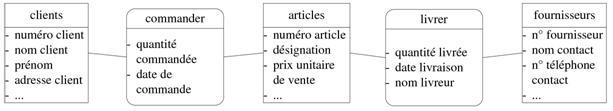
\includegraphics[width=0.9\linewidth]{attribut.jpg}
  \end{center}
  \begin{itemize}
    \item Le \emph{numéro article} et le \emph{prix unitaire} sont des attributs de l'entité \emph{articles},\\
      la \emph{quantité commandée} est un attribut de l'association \emph{commander}, etc.
    \item Une entité et ses attributs ne doivent traiter que d'un seul sujet
    \item[$\ra$] Mettre les informations relatives aux fournisseurs dans une entité \emph{fournisseurs} séparée
      plutôt que dans l'entité \emph{articles}
  \end{itemize}
\end{frame}

\begin{frame}
  \frametitle{Identifiant}
  \begin{itemize}
    \item Identifiant : attribut sans doublon qui identifie l'entité de manière unique
  \end{itemize}
  \begin{center}
    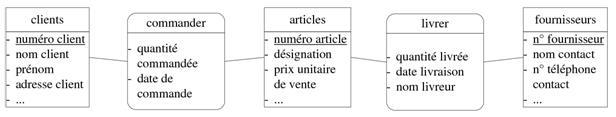
\includegraphics[width=0.9\linewidth]{identifiant.jpg}
  \end{center}
  \begin{itemize}
    \item Par convention, on souligne l'attribut identifiant sur le schéma
    \item En général, si il n'y a pas d'attribut adapté, on ajoute un numéro auto-incrémenté
    \item Une entité possède au moins un attribut (son identifiant)
    \item Une association peut être dépourvue d'attribut
  \end{itemize}
\end{frame}

%\subsection{Cardinalités}

\begin{frame}
  \frametitle{Cardinalités (1)}
  \begin{itemize}
    \item Cardinalité : pour un lien entre une entité et une association, elle précise le minimum et le maximum de
      fois qu'un individu de l'entité peut être concerné par l'association
  \end{itemize}
  \begin{center}
    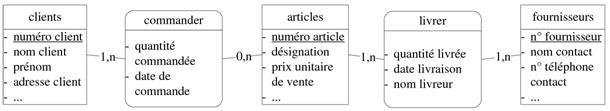
\includegraphics[width=0.9\linewidth]{cardinalites.jpg}
  \end{center}
  \begin{itemize}
    \item Exemple :
      \begin{itemize}
        \item Un \emph{client} a au moins commandé un \emph{article} et peut en commander $n$
        \item Un \emph{article} peut avoir été commandé entre $0$ et $n$ fois
      \end{itemize}
  \end{itemize}
\end{frame}

\begin{frame}
  \frametitle{Cardinalités (2)}
  \begin{center}
    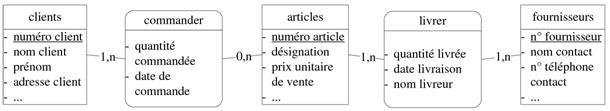
\includegraphics[width=0.9\linewidth]{cardinalites.jpg}
  \end{center}
  \begin{itemize}
    \item Une cardinalité minimale de $0$ : les individus de l'entité peuvent exister seuls
    \item Une cardinalité minimale de $1$ : les individus de l'entité ont besoin de l'association pour exister
      (un client n'existe que si il a commandé)
    \item Une cardinalité maximale de $1$ : les individus de l'entité sont reliés au maximum à un autre individu
      de l'autre entité
    \item Une cardinalité maximale de $n$ : les individus de l'entité peuvent reliés à plusieurs individus de
      l'autre entité
    \item En général, on n'utilise pas de cardinalités minimales de plus de $1$ car elle n'auront pas d'impact
      par la suite (cf. modèle relationnel)
  \end{itemize}
\end{frame}

%\subsection{Associations}

\begin{frame}
  \frametitle{Associations plurielles}
  \begin{itemize}
    \item Deux mêmes entités peuvent être plusieurs fois en association
  \end{itemize}
  \begin{center}
    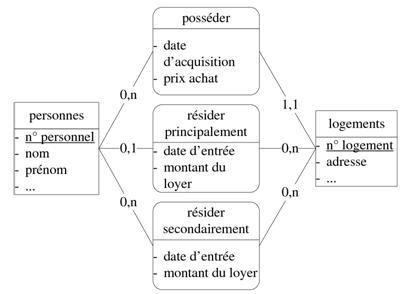
\includegraphics[width=0.6\linewidth]{associations_plurielles.jpg}
  \end{center}
  \begin{itemize}
    \item Permet d'indiquer des liens de différentes natures
  \end{itemize}
\end{frame}

\begin{frame}
  \frametitle{Association réflexive}
  \begin{itemize}
    \item Une association peut être reliée plusieurs fois avec la même entité
  \end{itemize}
  \begin{center}
    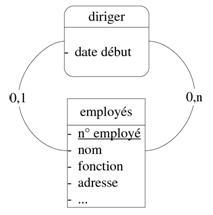
\includegraphics[width=0.35\linewidth]{association_reflexive.jpg}
  \end{center}
  \begin{itemize}
    \item Un employé est dirigé par un autre employé (sauf le directeur général)
    \item Un employé peut diriger plusieurs autres employés
  \end{itemize}
\end{frame}

\begin{frame}
  \frametitle{Associations non binaires (1)}
  \begin{itemize}
    \item Une entité avec associations de cardinalités maximales 1 au centre et n à l'extérieur peut-être
      remplaçée par une association avec les cardinalités extérieures
  \end{itemize}
  \begin{center}
    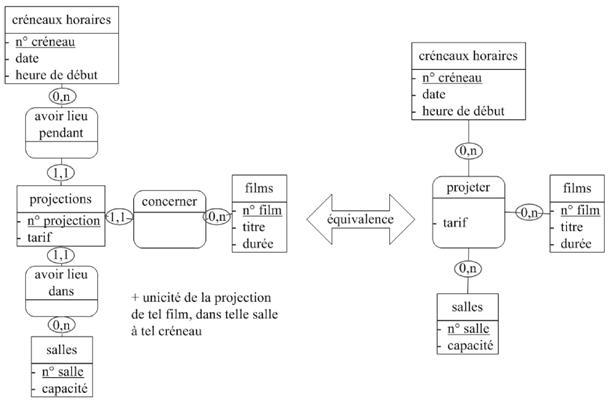
\includegraphics[width=0.8\linewidth]{assocation_ternaire.jpg}
  \end{center}
\end{frame}

\begin{frame}
  \frametitle{Associations non binaires (2)}
  \begin{itemize}
    \item Passer par un schéma entités-associations avec des associations binaires dans un premier temps
      permet d'éviter les association $n$-aires abusives (cardinalités non adéquates)
  \end{itemize}
  \begin{center}
    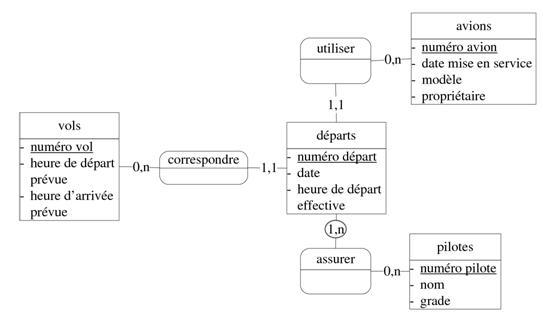
\includegraphics[width=0.8\linewidth]{assocation_ternaire2.jpg}
  \end{center}
\end{frame}

\begin{frame}
  \frametitle{Associations non binaires (3)}
  \begin{itemize}
    \item Une association peut être branchée à plus de trois entités
  \end{itemize}
  \begin{center}
    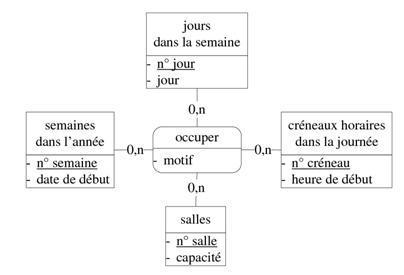
\includegraphics[width=0.6\linewidth]{assocation_quaternaire.jpg}
  \end{center}
\end{frame}


\begin{frame}
  \frametitle{Méthodologie}
  \begin{enumerate}
    \item Identifier les entités en présence
    \item Lister leurs attributs
    \item Ajouter les identifiants
    \item Établir les associations binaires entre les entités
    \item Lister leurs attributs
    \item Calculer les cardinalités
    \item Vérifier les règles de normalisation
    \item Effectuer les corrections nécessaires
  \end{enumerate}
\end{frame}
